\documentclass[a4paper,10pt]{article}
\usepackage[utf8]{inputenc}
\usepackage{listings}
\usepackage{graphicx}
\usepackage{subcaption}
\usepackage{adjustbox}
\usepackage{hyperref}
\usepackage{imakeidx}
\usepackage{hyperref}

\title{Compte rendu TP : Architecture logicielle}
\date{29/05/21}
\author{Hamze Al-Rasheed - Nicolas Commandeur - Benjamin Verdant - Robin Wagner}

\begin{document}
    \maketitle
    \pagenumbering{gobble}
    \newpage
    \tableofcontents
    \newpage
    \pagenumbering{arabic}
    
    \section{Sujet}
        Le principe du tp est de concevoir l'architecture d'un système de contrôle d'accès à un ensemble de bâtiments.
    
        Un bâtiment possède un nom ainsi que des informations. Les informations sont :
        \begin{itemize}
            \item la liste des portes du bâtiment
            \begin{itemize}
                \item Le nom de la porte    \newline
                \textit{ex : Porte sud, 8A-44, etc}
                \item L'id de la badgeuse d'entrée et de sortie de la porte
                \newline
                Impair pour entrer et pair pour sortir \newline
                \textit{ex : 11 pour entrer dans le bâtiment 1 et 12 pour en sortir}
                \item La liste des cartes autorisées ou non 
                \newline
                \textit{ex : Badgeuse 11 : carte 1 autorisée, carte 2 non autorisée, etc}
                \item L'état de la porte
                \newline
                \textit{ex : Ouvert ou fermé}
            \end{itemize}
        \end{itemize}
        
        Les utilisateurs ont chacun une \textbf{carte} qui a un \textbf{id} unique et le nom du détenteur de celle-ci.
        \newline
        \textit{ex : carte 1 $\Rightarrow$ Livai, carte 2 $\Rightarrow$ Eren }

        Pour accéder à un bâtiment ou à une salle, un utilisateur doit poser sa carte sur la badgeuse.
        \newline
        \par Si la personne \underline{est autorisée} à entrer dans le bâtiment alors, la porte s'ouvre et une lumière verte s'affiche pendant \textbf{15 secondes} et la porte reste ouverte pendant le \textbf{même temps}.
        \newline
        Si la personne n'est pas autorisée à entrer dans le bâtiment, une lumière rouge s'allume sur celle-ci.
        \newline
        \par
        Quand une personne ouvre une porte, un laser se situe juste après celle-ci, pour compter le nombre de personne qui passe. Plusieurs cas possibles :
        \begin{itemize}
            \item Une seule personne passe $\Rightarrow$ la personne qui a ouvert la porte est enregistrée dans le bâtiment et une trace de son passage est inscrit dans le log des passages.
            \item Plusieurs personnes passent $\Rightarrow$ une alarme retentit
            \item Personne ne passe $\Rightarrow$ rien ne se passe
        \end{itemize}

        Dans tous les cas, la porte se ferme au bout de \textbf{15 secondes}
        \newline

        \par En cas d'un incendie, toutes les portes sont débloquées et on inscrit dans un fichier toutes les personnes dans les bâtiments.
        \pagebreak

    \section{Prémice}
    Tout d'abord, nous avons analysé le sujet puis nos avons fait un diagramme de classe et un prototype d'un diagramme de séquence. Ceux-ci ont servi de base et ont été modifiés au fur et à mersure.

    \begin{figure}[h]
        \begin{subfigure}{1.0\textwidth}
            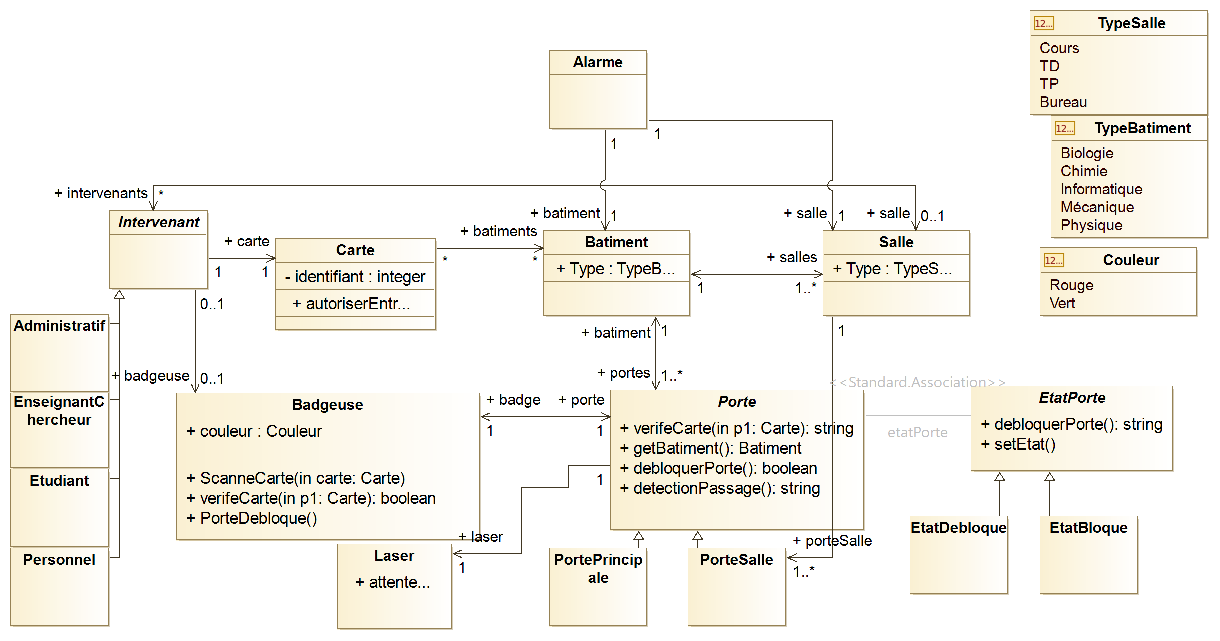
\includegraphics[width=1.2\linewidth, height=8cm]{image/classe.png}
             \caption{Diagramme de classe}
             \label{fig:classe}
        \end{subfigure}

    \end{figure}


    \begin{figure}[h]
        \begin{subfigure}{1.0\textwidth}

        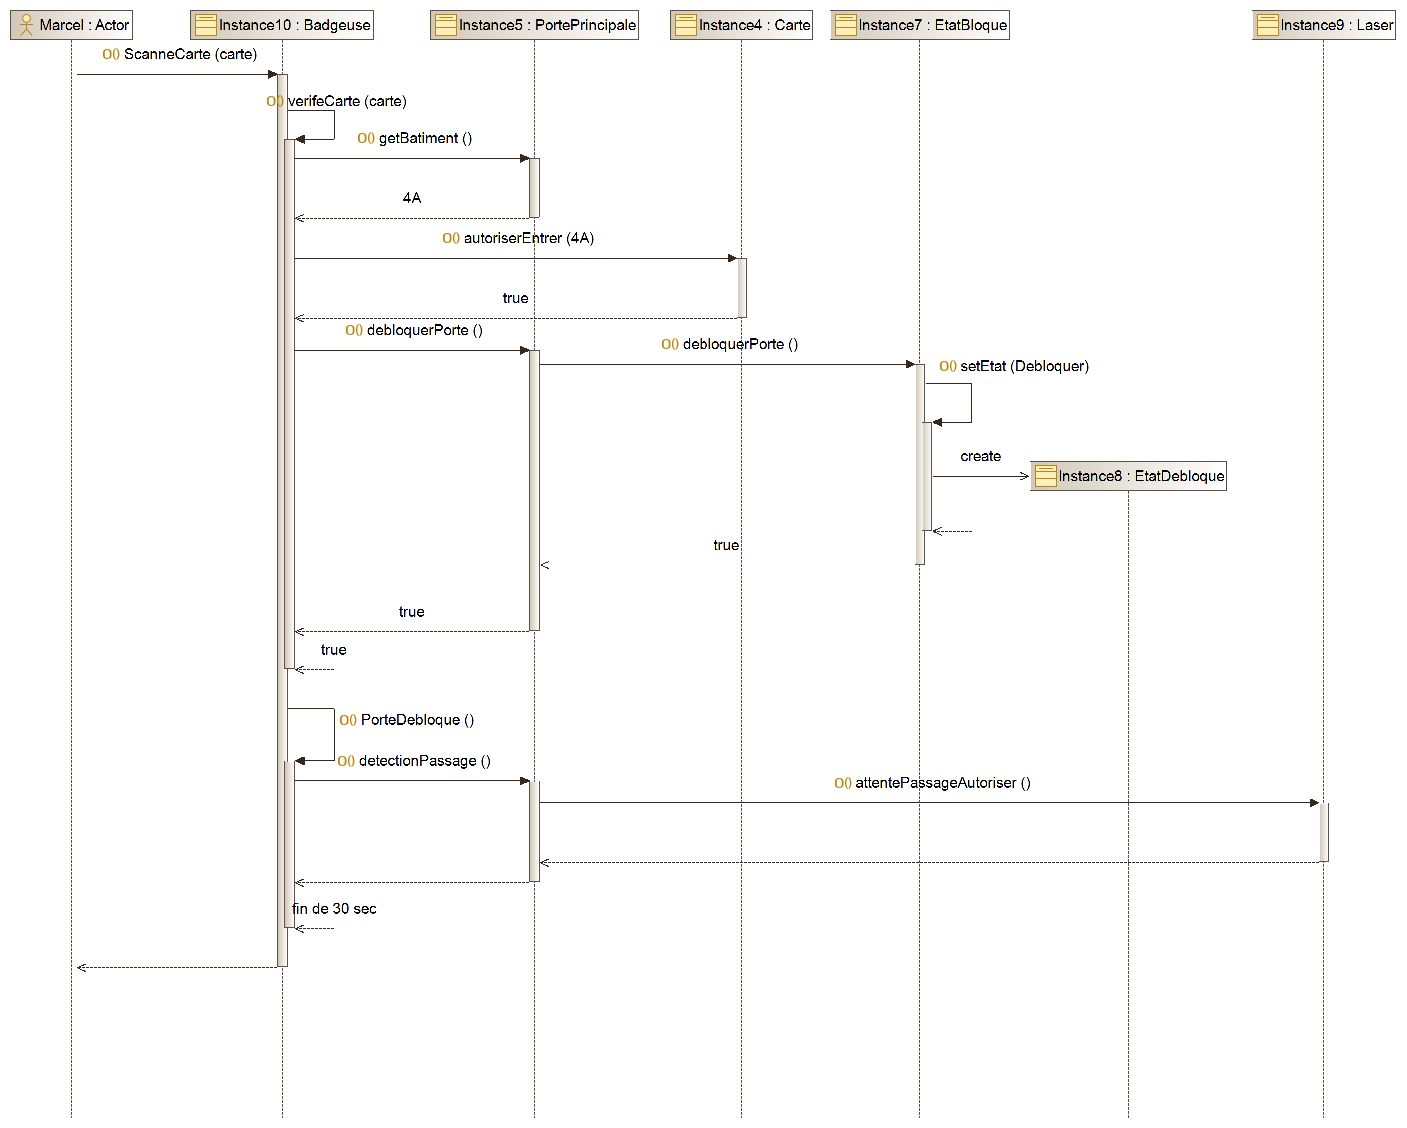
\includegraphics[width=1\linewidth, height=12cm]{image/sequence.png}   
        \caption{Diagramme en séquence}
        \label{fig:sequence}
        \end{subfigure}

    \end{figure}

    \clearpage
    
    
    \section{Architecture utilisée}

    Nous sommes partis sur un architecture à base de tuple comme celle vue en cours, et pour cela, nous avons décidé de réaliser une classe dédié : \textit{espaceDeTuples}. Voici sa définition :
    \begin{lstlisting}[language=Python]
class espaceDeTuples():
    def OUT(self, element):
        self.listeTuples.append(element)

    def IN(self, element, tab):
        resTemp = self.existe(element, tab)
        res = list()
        for index in tab:
            res.append(resTemp[index])
        self.listeTuples.remove(resTemp)
        return res

    def RD(self, element, tab):
        resTemp = self.existe(element, tab)
        res = list()
        for index in tab:
            res.append(resTemp[index])
        return res

    def ADD(self, element, tab):
        resTemp = self.existe(element, tab)
        index = self.listeTuples.index(resTemp)
        listTuple = list(self.listeTuples[index])
        for i in tab:
            listTuple[i] = element[i]
        self.listeTuples[index] = tuple(listTuple)

    def INUNBLOCKED(self, element, tab):
        resTemp = self.existeNonBloquant(element, tab)
        if resTemp is None:
            return None
        res = list()
        for index in tab:
            res.append(resTemp[index])
        self.listeTuples.remove(resTemp)
        return res

    def existe(self, template, tab):
        tuplePossible = []
        while (True):
            for tupleI in self.listeTuples:
                flag = True
                if len(tupleI) == len(template):
                    for i in range(len(template)):
                        if type(template[i]) != type(tupleI[i]):
                            flag = False
                    if flag:
                        tuplePossible.append(tupleI)
            for tupleI in tuplePossible:
                allIndex = list(range(len(tupleI)))
                for i in tab:
                    for j in allIndex:
                        if i == j:
                            allIndex.remove(j)
                flag = True
                for i in allIndex:
                    if template[i] != tupleI[i]:
                        flag = False
                if flag:
                    return tupleI

    def existeNonBloquant(self, template, tab):
        tuplePossible = []
        for tupleI in self.listeTuples:
            flag = True
            if len(tupleI) == len(template):
                for i in range(len(template)):
                    if type(template[i]) != type(tupleI[i]):
                        flag = False
                if flag:
                    tuplePossible.append(tupleI)
            for tupleI in tuplePossible:
                allIndex = list(range(len(tupleI)))
                for i in tab:
                    for j in allIndex:
                        if i == j:
                            allIndex.remove(j)
                flag = True
                for i in allIndex:
                    if template[i] != tupleI[i]:
                        flag = False
                if flag:
                    return tupleI

    def __init__(self):
        self.listeTuples = list()

    \end{lstlisting}
    Cette classe implémente les différentes interactions dont notre programme avait besoin. 

    \textbf{Ps : } Problème dans la fonction \textit{existe} qui a une boucle \verb|while True| et qui est la cause principale des problèmes rencontrés. Voir \nameref{difficulty}.

    
    \par Nous avons choisi seulement cette implémentation car elle remplit à elle seule les fonctionnements nécessaires au TP.   

    \pagebreak
    \section{Choix technologiques}
    Nous avons décidé d'utiliser python car celui-ci :
    \begin{itemize}
        \item Possède déjà une structure de tuples que nous avons utilisé dans la partie précédente
        \item Threading simple à implémenter
        \item Interface graphique simple à implémenter (Kivy)
        \item Pas trop lourd et rapide d'éxecution
    \end{itemize} 

    Dans notre TP, les espaces de tuples sont représentés par une \textbf{variable globale}. Dans le système final, cet espace serait représenté par une base de données. Chaque \textbf{agent} est représenté par un \textbf{Thread} dont la mémoire est partagée avec tous les autres Threads qui représentent les autres agents.

    \vspace{5mm} 

    La classe badgeuse est représenté par :

    \begin{itemize}
        \item lecteurCarte : dépose un tuple dans l'espace de tuple
        \item verifCarte : autorise la personne à entrer dans le bâtiment
        \item scanCarte : lance la détection et l'allumage des leds
        \item lumiereVerte : s'allume lorsque la personne est autorisée
        \item lumiereRouge : s'allume lorsque la personne n'est pas autorisée
        \item detectionPassage : le capteur dépose dans la base de tuple un tuple lorsque qu'il détecte lorsqu'une personne passe
        \item etatPorte : permet d'ouvrir une porte et de la fermer. En cas d'incendie, ferme toutes les portes.
    \end{itemize}

    Nous avons aussi des agents pour les fonctions secondaires : 
    \begin{itemize}
        \item declencheAlarme : Souleve l'alerte si il y a plus d'une personne qui passe
        \item incendie : le capteur d'incendie dépose un tuple qui est détecté par cet agent va déclencher une alarme.
    
    \end{itemize}
        
    \pagebreak
    \section{Petit pas pour l'homme}
    Nous avons décidé alors de commencer par l'agent qui permettait de scanner une carte, qui servira de \textit{core} aux restes des agents. Tout d'abord, nous avons fait un exemple en langage algorithmique :
    \begin{figure}[h]
        \begin{subfigure}{1.0\textwidth}
            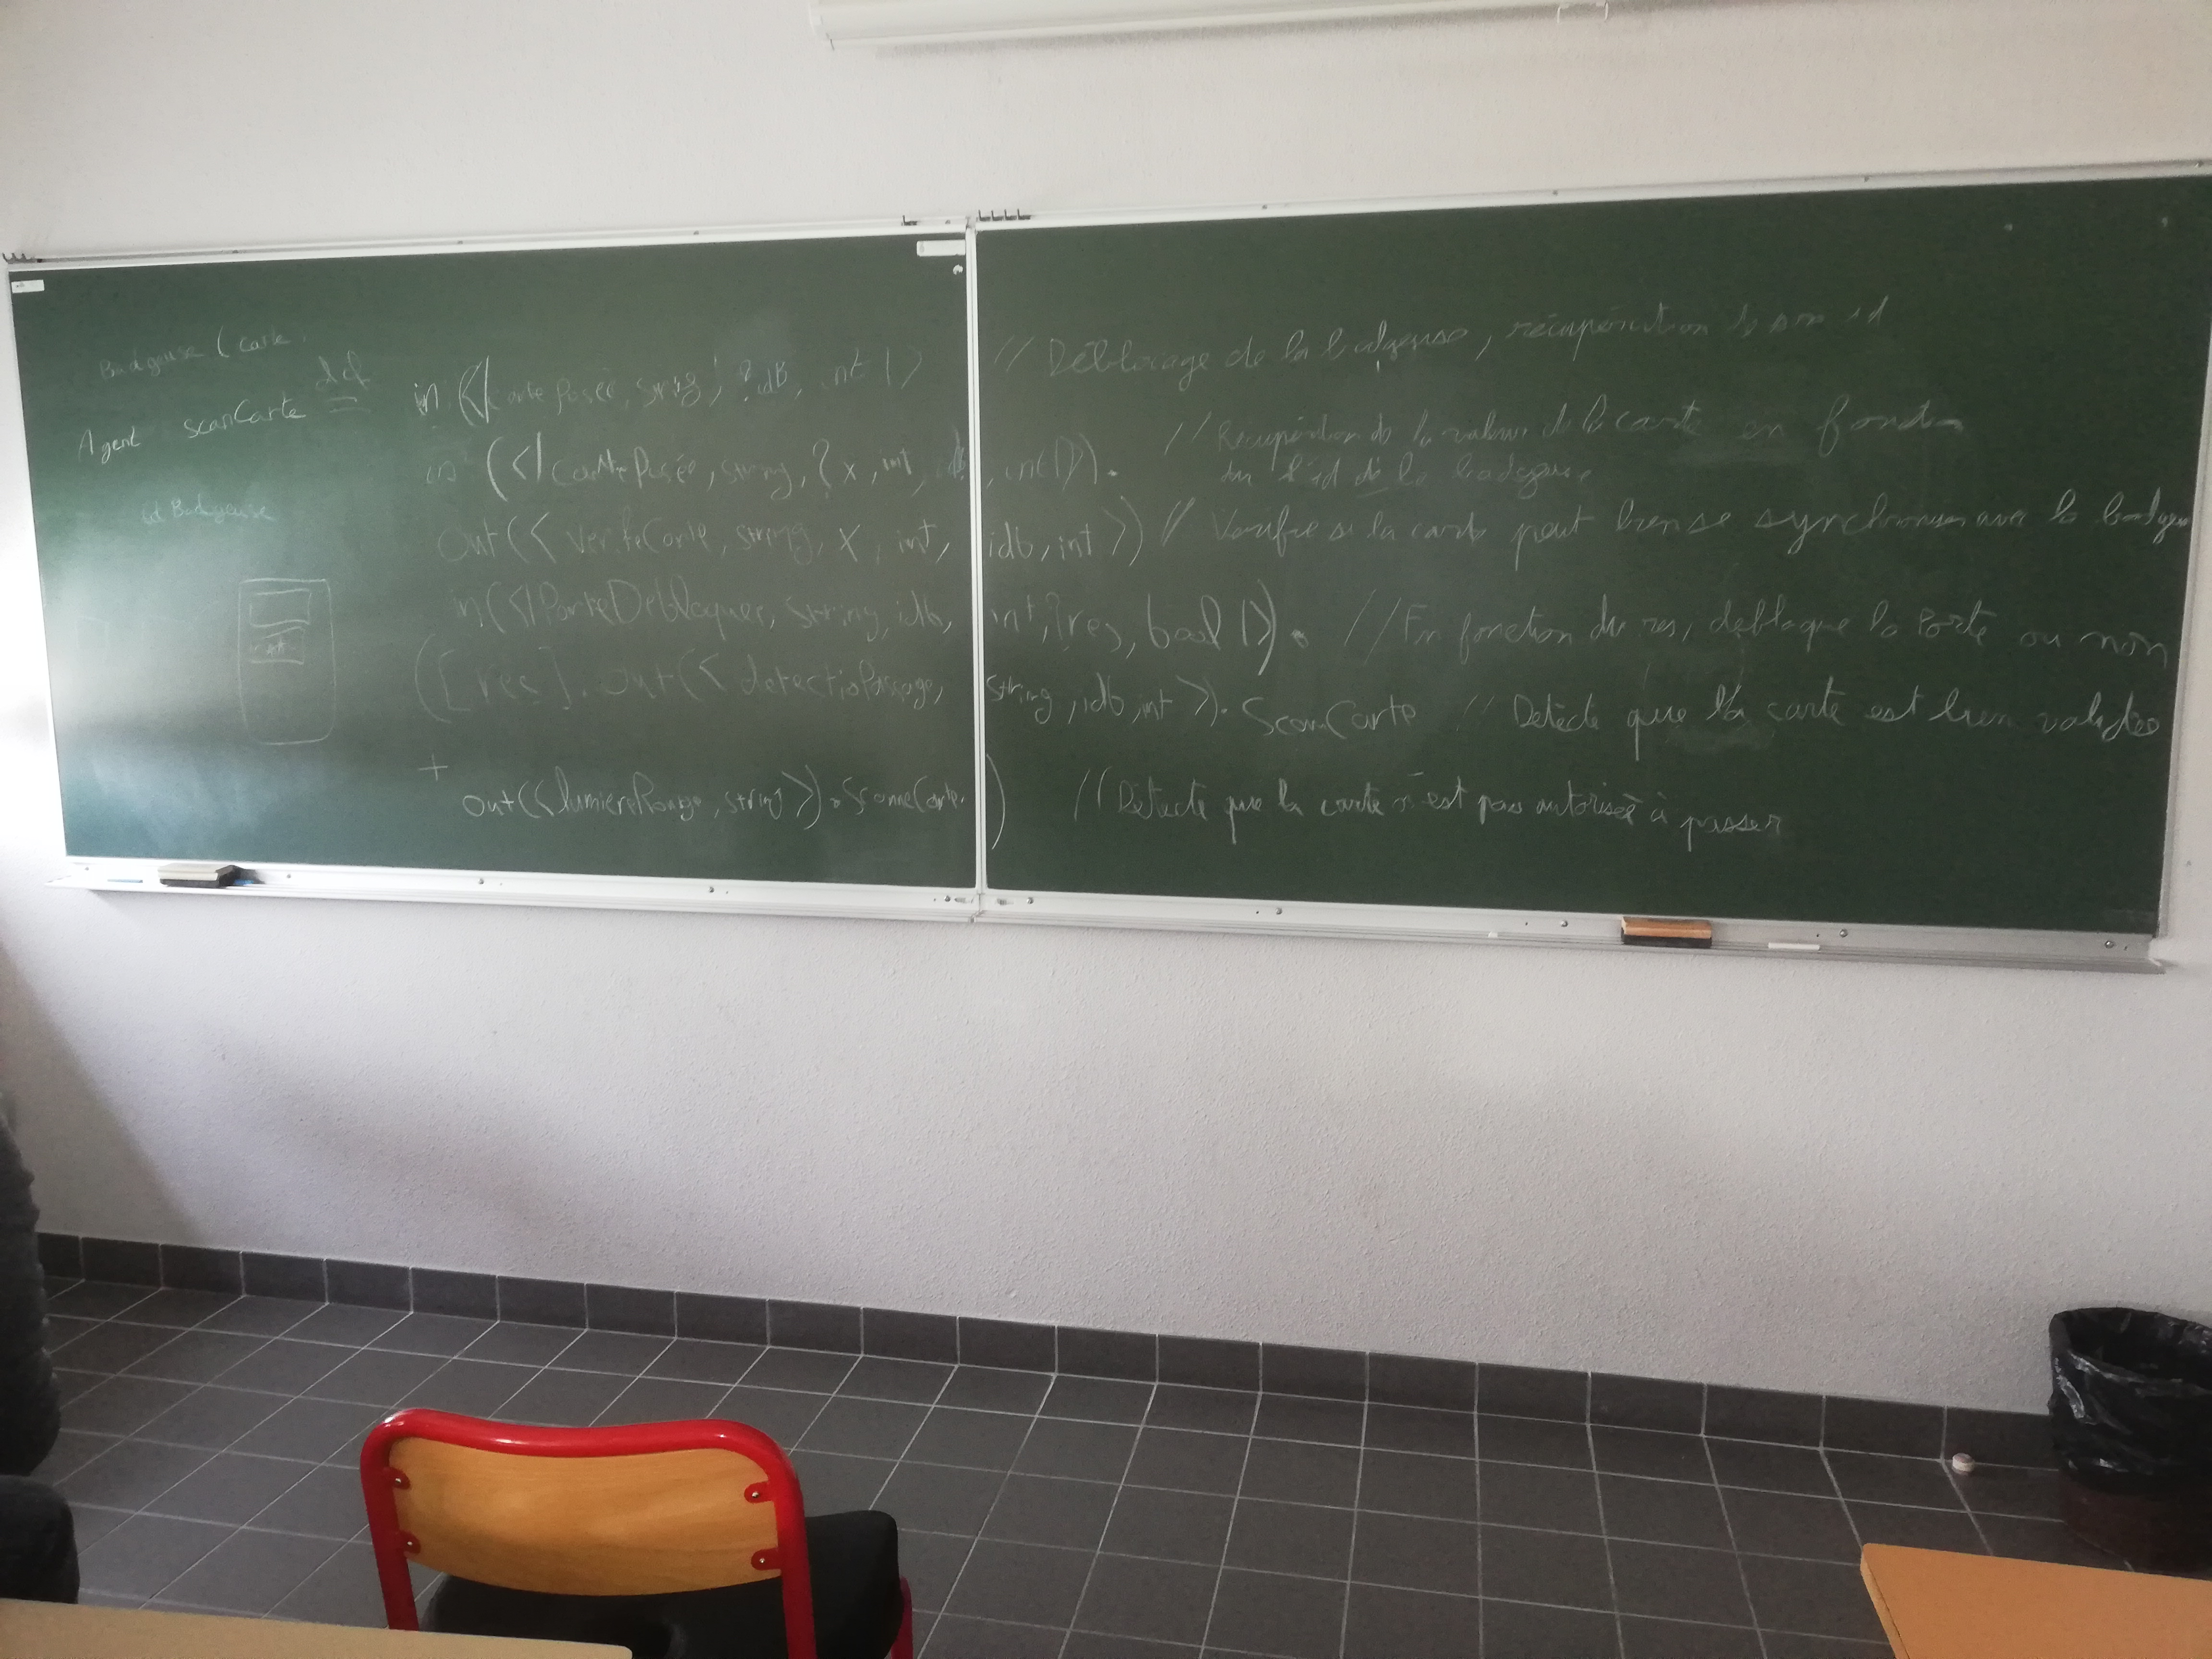
\includegraphics[width=1.2\linewidth, height=8cm]{image/tableau.jpg}
             \caption{1er jet}
             \label{fig:tableau}
        \end{subfigure}
    \end{figure}

    Assez difficile au début, mais petit à petit comme l'oiseau qui fait son nid, cet agent nous a bien servi pour le reste.

    \pagebreak
    \section{Grand pas pour l'humanité}
    Nous avons ensuite réalisé les autres agents. Nous les avons testé un par un, puis ensemble. Nous avons dû créer des agents spécialement pour l'interface, pour avoir un rendu direct avec l'espace de tuple.

    \begin{figure}[h]
        \begin{subfigure}{1.0\textwidth}
            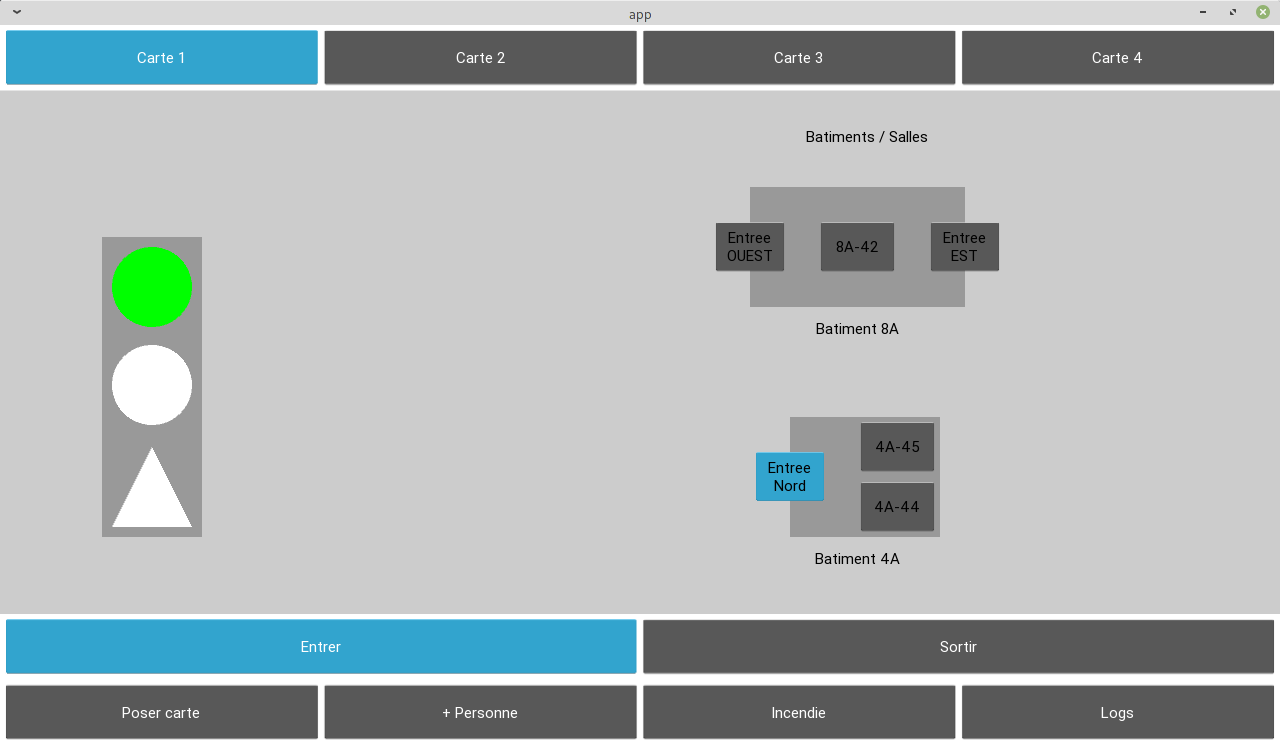
\includegraphics[width=1.0\linewidth, height=6cm]{image/interface-1.png}
             \caption{Interface grapique avec Kivy}
             \label{fig:interface1}
        \end{subfigure}
        \begin{subfigure}{1.0\textwidth}
            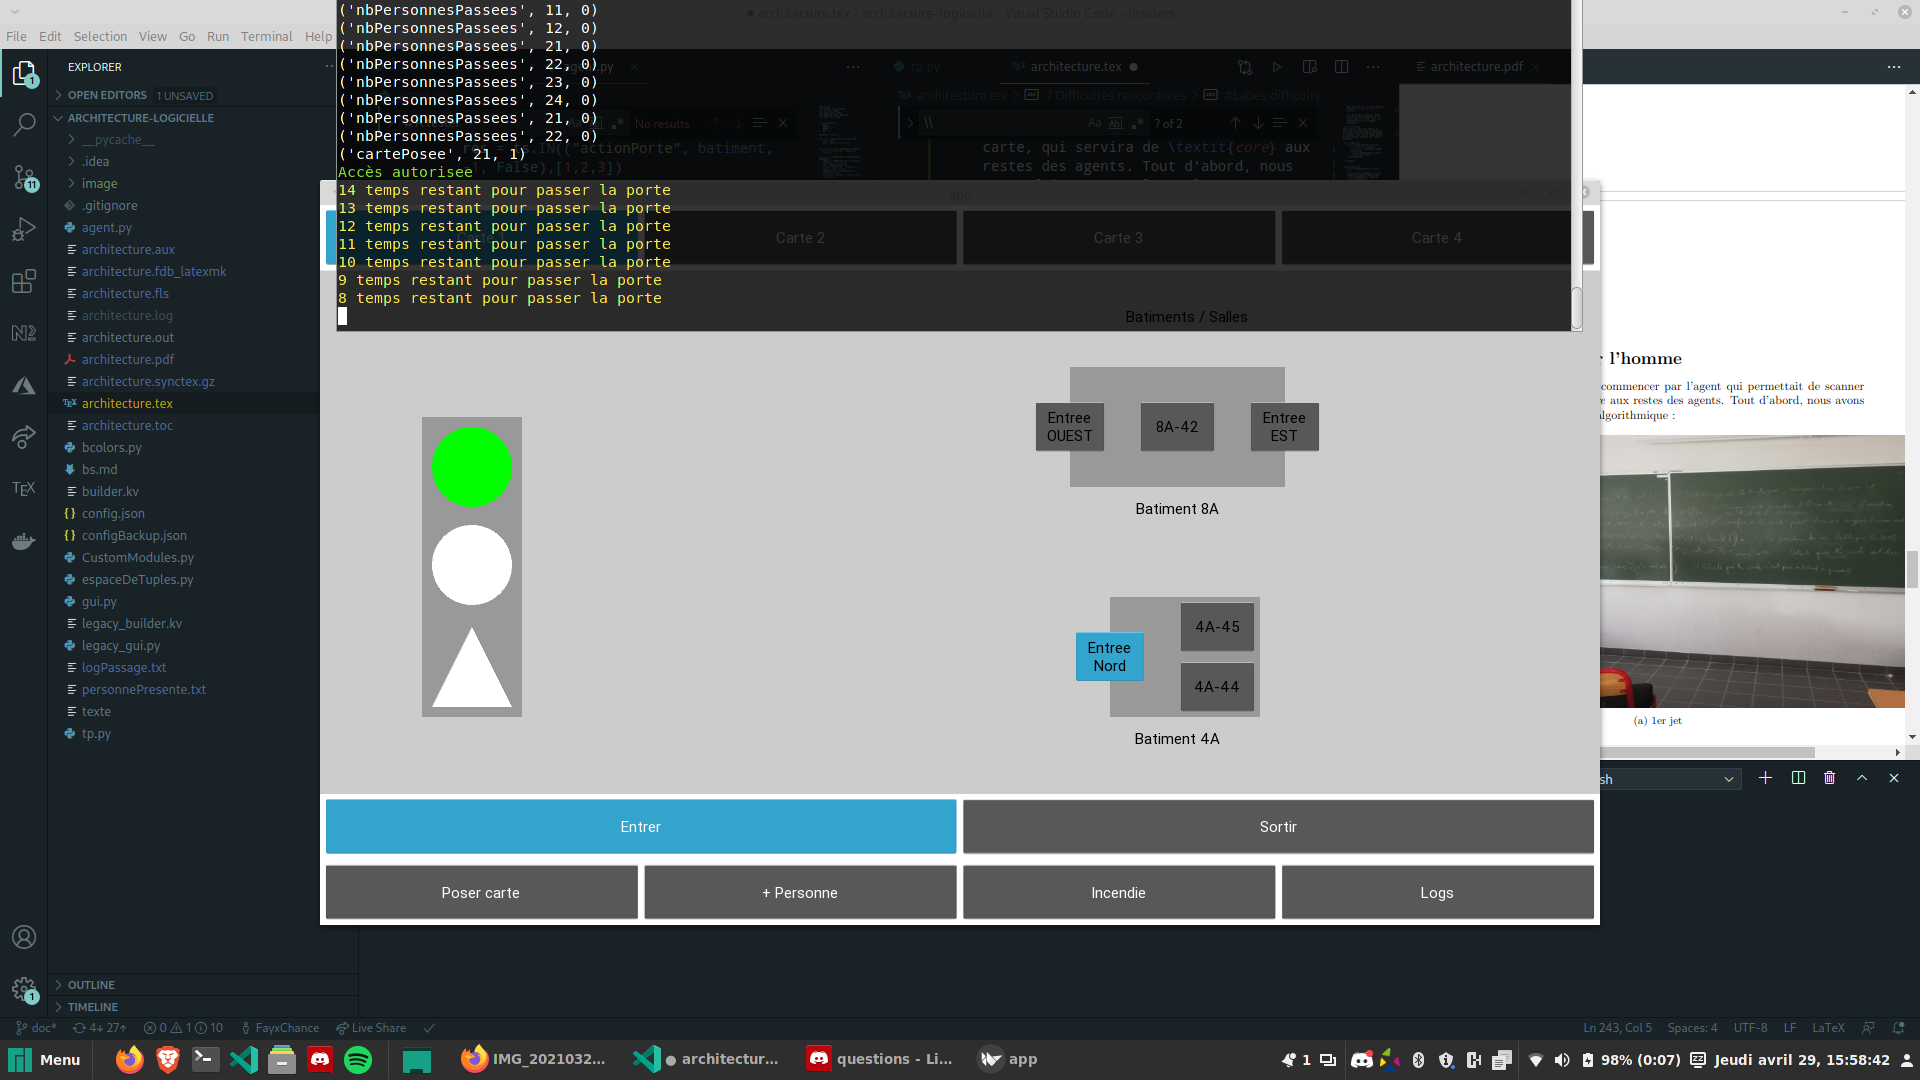
\includegraphics[width=1.0\linewidth, height=6cm]{image/interface-2.png}
             \caption{Interface avec la console qui affiche le temps}
             \label{fig:tableau}
        \end{subfigure}
    \end{figure}
    
    \pagebreak
    \section{Difficultés rencontrées}
    \label{difficulty}
    \par Au debut de notre travail nous avons voulu faire le TP avec JAVA car Modelio nous permettait de créer un diagramme d'objet et des diagrammes de séquences que nous pouvions directement exporter en code JAVA.
    Cependant nous nous sommes rendu compte que JAVA n'était pas une bonne idée puisque, lui-même, consomme déjà beaucoup de mémoire pour éxecuter un programme.
    De plus l'architecture créée par Modelio ne convenait pas au sujet et aux objectifs du TP. Après avoir pris du recul nous avons décidé d'utiliser Python car c'est un langage adapté pour faire une architecture à base de tuples.
    \\
    \par
    La seconde difficulté qui nous est apparue est lors de l'assignation de nos fonctions sur des threads. Nous avons commencer à assigner les threads fonction par fonction et à les tester un par un pour vérifier qu'ils fonctionnaient correctement indépendement les uns des autres. Lorsque toutes les fonctions avaient été vérifiées nous avons commencé à faire tourner tous les threads en même temps. Mais, le programme avait un temps d'exécution beaucoup trop long pour pouvoir l'utiliser. Nous avions plus de \textbf{200} threads qui fonctionnaient les un en même temps que les autres. C'est pour cela, que nous avons minimisé le nombre de badgeuse, de bâtiment... lors de la démonstration.
    \\
    \par
     Ensuite nous avons eu des soucis lors de la création de l'inteface et avant tout pour l'imaginer. Il nous fallait une interface qui puisse interagir avec l'espace de tuple en temps réel et de façon intuitive.

    \pagebreak
    \section{Ce que nous avons appris}
    Pour conclure, trop de thread tue les threads. Les threads ont leur limite, il aurait été peut être plus judiceux de faire des processus, mais nous aurions dû changer la représentation de notre espace de tuple avec une base de données. Lier le backend avec l'interface tout en utilisant les tuples et composant connecteur pour les boutons.
\end{document}